\documentclass{article}
\usepackage[utf8]{inputenc}
\usepackage{amsmath}
\usepackage{amssymb}
\usepackage{amsfonts}
\usepackage{amssymb}
\usepackage{minted}
\usepackage{graphicx}
\graphicspath{ {img/} }
\usepackage{titlesec}
\usepackage[a4paper,margin=1in,footskip=0.25in]{geometry}
\usepackage{fancyhdr}
\pagestyle{fancy}
%basic page layout

%draw finite state machine
\usepackage{tikz}
\usetikzlibrary{arrows,automata}
\newcommand{\hwnumber}{1}
\newcommand{\Lcvy}{\mathcal{L}}
%header and footer settings
\lhead{Algorithms and Data Structure \hwnumber}
\chead{Yiping Deng}
\rhead{\today}

\titlelabel{\thetitle\enspace}

\begin{document}
\title{Algorithms and Data Structure \hwnumber}
\author{Yiping Deng}
\maketitle
\thispagestyle{fancy}
\section*{Problem 1}
General proof for limit implies asymptotic notation. \\
case 1:
\begin{align*}
    \lim_{n \to \infty} \frac{f(x)}{g(x)} = c \text{ s.t. } c > 0 \text{ and } c < \infty \implies \\
    \text{ for sufficiently large n,} | \frac{f(x)}{g(x)} - c | < \epsilon \implies \\
    c - \epsilon < \frac{f(x)}{g(x)} < c + \epsilon \implies \\
    c_1 < \frac{f(x)}{g(x)} < c_2 \implies \\
    c_1 g(x) < f(x) < c_2 g(x) \implies \\
    f \in \Theta(g)
\end{align*}
case 2:
\begin{align*}
    \lim_{n \to \infty} \frac{f(x)}{g(x)} = 0 \implies \\
    \text{ for sufficiently large n,} | \frac{f(x)}{g(x)}| < \epsilon \implies \\
    f(x) < \epsilon g(x) \text{ since f, g are positive by default, } \epsilon > 0 \text{, it holds for every }\epsilon \implies \\
    f \in o(g) \implies g \in \omega(f)
\end{align*}
case 3:
\begin{align*}
    \lim_{n \to \infty} \frac{f(x)}{g(x)} = \infty \implies \\
    \lim_{n \to \infty} \frac{g(x)}{f(x)} = 0 \implies \\
    \text{ for sufficiently large n,} | \frac{g(x)}{f(x)}| < \epsilon \implies \\
    g(x) < \epsilon f(x) \text{ since f, g are positive by default, } \epsilon > 0 \text{, it holds for every }\epsilon \implies \\
    g \in o(f) \implies f \in \omega(g)
\end{align*}
\subsection*{a)}
\begin{enumerate}
    \item $f \in \Theta(g)$ not true.
        $$ \lim_{n \to \infty} \frac{f(n)}{g(n)} = 0$$
    \item $f \in O(g)$ true.
        $$ \lim_{n \to \infty} \frac{f(n)}{g(n)} = 0 < \infty$$
    \item $f \in o(g)$ true.
        $$ \lim_{n \to \infty} \frac{f(n)}{g(n)} = 0$$
    \item $f \in \Omega(g)$ not true.
        $$ \lim_{n \to \infty} \frac{g(n)}{f(n)} = \infty$$
    \item $f \in \omega(g)$ not true.
        $$ \lim_{n \to \infty} \frac{g(n)}{f(n)} = \infty$$
    \item $g \in \Theta(f)$ not true.
        $$ \lim_{n \to \infty} \frac{g(n)}{f(n)} = \infty$$
    \item $g \in O(f)$ not true.
        $$ \lim_{n \to \infty} \frac{g(n)}{f(n)} = \infty$$
    \item $g \in o(f)$ not true.
        $$ \lim_{n \to \infty} \frac{g(n)}{f(n)} = \infty$$
    \item $g \in \Omega(f)$ true.
        $$ \lim_{n \to \infty} \frac{f(n)}{g(n)} = 0 < \infty$$
    \item $g \in \omega(f)$ true.
        $$ \lim_{n \to \infty} \frac{f(n)}{g(n)} = 0 < \infty$$
\end{enumerate}

\subsection*{b)}
$g(n)$ can rewrite as:
\begin{align*}
    g(n) &= n^{\frac{1}{2}}
\end{align*}
\begin{enumerate}
    \item $f \in \Theta(g)$ not true.
        $$ \lim_{ n \to \infty} \frac{f(n)}{g(n)} = \lim_{ n \to \infty} \frac{ 7 n^{0.7} }{ n^{0.5}} = \infty $$
    \item $f \in O(g)$ not true.
        $$ \lim_{ n \to \infty} \frac{f(n)}{g(n)} = \lim_{ n \to \infty} \frac{ 7 n^{0.7} }{ n^{0.5}} = \infty $$
    \item $f \in o(g)$ not true.
        $$ \lim_{ n \to \infty} \frac{f(n)}{g(n)} = \lim_{ n \to \infty} \frac{ 7 n^{0.7} }{ n^{0.5}} = \infty $$
    \item $f \in \Omega(g)$ true.
        $$ \lim_{ n \to \infty} \frac{g(n)}{f(n)} = \lim_{ n \to \infty} \frac{n^{0.5}}{ 7 n^{0.7}} = 0$$
    \item $f \in \omega(g)$ true.
        $$ \lim_{ n \to \infty} \frac{g(n)}{f(n)} = \lim_{ n \to \infty} \frac{n^{0.5}}{ 7 n^{0.7}} = 0$$
    \item $g \in \Theta(f)$ not true.
        $$ \lim_{ n \to \infty} \frac{f(n)}{g(n)} = \lim_{ n \to \infty} \frac{n^{0.5}}{ 7 n^{0.7}} = 0$$
    \item $g \in O(f)$ true.
        $$ \lim_{ n \to \infty} \frac{g(n)}{f(n)} = \lim_{ n \to \infty} \frac{n^{0.5}}{ 7 n^{0.7}} = 0$$
    \item $g \in o(f)$ true.
        $$ \lim_{ n \to \infty} \frac{g(n)}{f(n)} = \lim_{ n \to \infty} \frac{n^{0.5}}{ 7 n^{0.7}} = 0$$
    \item $g \in \Omega(f)$ not true.
        $$ \lim_{ n \to \infty} \frac{f(n)}{g(n)} = \lim_{ n \to \infty} \frac{7 n^{0.7} }{ n^{0.5}} = \infty $$
    \item $g \in \omega(f)$ not true.
        $$ \lim_{ n \to \infty} \frac{f(n)}{g(n)} = \lim_{ n \to \infty} \frac{7 n^{0.7} }{ n^{0.5}} = \infty $$
\end{enumerate}

\subsection*{c)}
\begin{enumerate}
    \item $f \in \Theta(g)$ not true.
        $$ \lim_{n \to \infty} \frac{f(n)}{g(n)} = \lim_{n \to \infty} \frac{ n^2 / log(n)}{n log(n)} = \lim_{n \to \infty} \frac{ n / log(n) }{ log(n)} =
        \lim_{n \to \infty} \frac{n}{ log^2(n)} = \infty $$
    \item $f \in O(g)$ not true.
        $$ \lim_{n \to \infty} \frac{f(n)}{g(n)} = \lim_{n \to \infty} \frac{ n^2 / log(n)}{n log(n)} = \lim_{n \to \infty} \frac{ n / log(n) }{ log(n)} =
        \lim_{n \to \infty} \frac{n}{ log^2(n)} = \infty $$
    \item $f \in o(g)$ not true.
        $$ \lim_{n \to \infty} \frac{f(n)}{g(n)} = \lim_{n \to \infty} \frac{ n^2 / log(n)}{n log(n)} = \lim_{n \to \infty} \frac{ n / log(n) }{ log(n)} =
        \lim_{n \to \infty} \frac{n}{ log^2(n)} = \infty $$
    \item $f \in \Omega(g)$ true.
        $$ \lim_{n \to \infty} \frac{g(n)}{f(n)} = \lim_{n \to \infty} \frac{1}{f(n)/g(n)} = 0 $$
    \item $f \in \omega(g)$ true.
        $$ \lim_{n \to \infty} \frac{g(n)}{f(n)} = \lim_{n \to \infty} \frac{1}{f(n)/g(n)} = 0 $$
    \item $g \in \Theta(f)$ not true.
        $$ \lim_{n \to \infty} \frac{f(n)}{g(n)} = \lim_{n \to \infty} \frac{ n^2 / log(n)}{n log(n)} = \lim_{n \to \infty} \frac{ n / log(n) }{ log(n)} =
        \lim_{n \to \infty} \frac{n}{ log^2(n)} = \infty $$
    \item $g \in O(f)$ true.
        $$ \lim_{n \to \infty} \frac{g(n)}{f(n)} = \lim_{n \to \infty} \frac{1}{f(n)/g(n)} = 0 $$
    \item $g \in o(f)$ true.
        $$ \lim_{n \to \infty} \frac{g(n)}{f(n)} = \lim_{n \to \infty} \frac{1}{f(n)/g(n)} = 0 $$
    \item $g \in \Omega(f)$ not true.
        $$ \lim_{n \to \infty} \frac{f(n)}{g(n)} = \lim_{n \to \infty} \frac{ n^2 / log(n)}{n log(n)} = \lim_{n \to \infty} \frac{ n / log(n) }{ log(n)} =
        \lim_{n \to \infty} \frac{n}{ log^2(n)} = \infty $$
    \item $g \in \omega(f)$ not true.
        $$ \lim_{n \to \infty} \frac{f(n)}{g(n)} = \lim_{n \to \infty} \frac{ n^2 / log(n)}{n log(n)} = \lim_{n \to \infty} \frac{ n / log(n) }{ log(n)} =
        \lim_{n \to \infty} \frac{n}{ log^2(n)} = \infty $$
\end{enumerate}

\subsection*{d)}
\begin{enumerate}
    \item $f \in \Theta(g)$ not true.
        $$ \lim_{n \to \infty} \frac{f(n)}{g(n)} = \lim_{n \to \infty} \frac{log(3n)}{9 log(n)} (log(3n))^2 = \infty $$
    \item $f \in O(g)$ not true.
        $$ \lim_{n \to \infty} \frac{f(n)}{g(n)} = \lim_{n \to \infty} \frac{log(3n)}{9 log(n)} (log(3n))^2 = \infty $$
    \item $f \in o(g)$ not true.
        $$ \lim_{n \to \infty} \frac{f(n)}{g(n)} = \lim_{n \to \infty} \frac{log(3n)}{9 log(n)} (log(3n))^2 = \infty $$
    \item $f \in \Omega(g)$ true.
        $$ \lim_{n \to \infty} \frac{g(n)}{f(n)} = \lim_{n \to \infty} \frac{1}{f(n)/g(n)} = 0 $$
    \item $f \in \omega(g)$ true.
        $$ \lim_{n \to \infty} \frac{g(n)}{f(n)} = \lim_{n \to \infty} \frac{1}{f(n)/g(n)} = 0 $$
    \item $g \in \Theta(f)$ not true.
        $$ \lim_{n \to \infty} \frac{g(n)}{f(n)} = \lim_{n \to \infty} \frac{1}{f(n)/g(n)} = 0 $$
    \item $g \in O(f)$ not true.
        $$ \lim_{n \to \infty} \frac{g(n)}{f(n)} = \lim_{n \to \infty} \frac{1}{f(n)/g(n)} = 0 $$
    \item $g \in o(f)$ not true.
        $$ \lim_{n \to \infty} \frac{g(n)}{f(n)} = \lim_{n \to \infty} \frac{1}{f(n)/g(n)} = 0 $$
    \item $g \in \Omega(f)$
        $$ \lim_{n \to \infty} \frac{f(n)}{g(n)} = \lim_{n \to \infty} \frac{log(3n)}{9 log(n)} (log(3n))^2 = \infty $$
    \item $g \in \omega(f)$
        $$ \lim_{n \to \infty} \frac{f(n)}{g(n)} = \lim_{n \to \infty} \frac{log(3n)}{9 log(n)} (log(3n))^2 = \infty $$
\end{enumerate}

\section*{Problem 2}
\subsection*{(a)} Implementation of selection sort in Scala\\
File 1: SelectionSort.scala
\inputminted{Scala}{code/src/main/scala/SelectionSort.scala}
File 2: Timer.scala
\inputminted{Scala}{code/src/main/scala/Timer.scala}
File 3(Unit test): SelectionSortTest.scala
\inputminted{Scala}{code/src/test/scala/SelectionSortTest.scala}

The Scala code successfully passed the test case. To compile, you can simply execute under code folder
\begin{minted}{Bash}
    # sbt
    > compile
    > test
\end{minted}
\subsection*{(b)}
Loop invariant: \\
\textbf{Initialization:} Consider the case when $unsortedIdx == 1$. Under such case, the subarray contains only one element,
the minimum of the original array. It is sorted, and its order(or index) will remain unchanged.
\\
\textbf{Maintanence:} Assuming before entering the loop, the subarray $A$ indexed from $0$ to $unsortedIdx - 1$ is sorted,
and all the element in the subarray is smaller than \textbf{any} elements in the remaining subarray $S \backslash A$.
Thus, upon execution of the loop, we have $ A = A \cup \{min(S \backslash A)\} $.
By the assumption, the new element in the subarray $ A $ is the biggest one. Hence,
the ordering of A remains unchanged. \\
\textbf{Termination:} Again, loop invariant is satisfied. When terminated, applying  $ A = A \cup \{min(S \backslash A)\} $, we have a sorted array.
\subsection*{(c)}
The code above, upon running, will generate the best and the worst case.
And it will feed into the function and note the running time. \\
Best case example: 2145757357 2146074127 2146212738 2146443596 2147032252 \\
Best case is generated by sorting. \\
Worst case example:  100 99 98 97 96 95 \\
Worst case is generated by sorting and reverse the array. \\
Note that best case and worst case is asympototically equivalent. Since the number of comparision
is the same. The only difference is on swap operation, which is minimal(number of swap operation
is linear)

\subsection*{(d)}
The data generated by executing the program is
\inputminted{Python}{plot.py}
First argument is the size of the dataset, second argument is the running time in millosecond.
Let's draw the graph and visualize. \\
Green is the Worst case.
Blue is the Best case.
Red is the Average case. \\
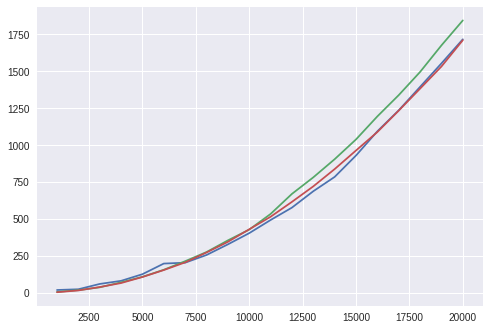
\includegraphics[scale=0.7]{plot.png}

\subsection*{(e)}
Interpretation:
The difference between three cases is minimal.
This algorithm can be modeled by the number of comparision made in the process of sorting.
In a array of size $ n $, in the $ i^{th} $ loop, the number of comparision in indexOfMin function
is $n - i + 1$, and we perform it $ n $ times. The total comparision is:
$$
Comparison = \sum_{i = 1}^{n} (n - i + 1) = \frac{n ( n + 1)}{2} \in O(n^2)
$$
which clearly explains the graph. It is quadratic.
The reason between best case and the worst case performance is the assignment in the min function and the swap operation.
\end{document}
